\section{Latch Etapa de Ejecuci\'on - Etapa de memoria}

Esta latch separa las de ejecuci\'on con la etapa de memoria.
\begin{figure}[H]
\centering
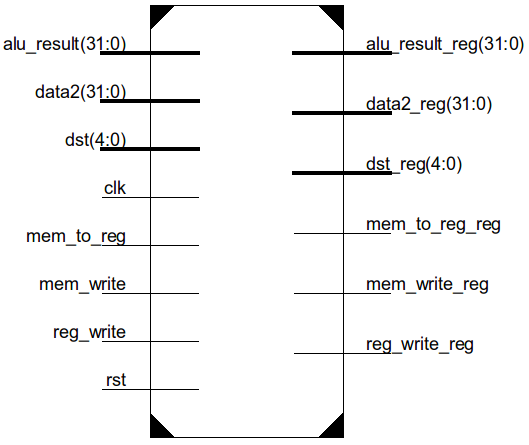
\includegraphics[scale=0.35]{img/latch_ex_m}
\caption{Latche Etapa de ejecucion - Etapa Memoria}
\label{fig:latch_ex_mem}
\end{figure}
Tiene como entradas:
\begin{itemize}
  \item \textbf{alu\_result}: Bus de 32 bits que tiene el resultado de la operaci\'on que se realizo en la ALU.
  \item \textbf{data2}: Bus de 32 bits, es pasado por esta etapa directamente desde el latch anterior para las instrucciones que tiene que escribir en la etapa de memoria justamente la memoria de datos, la escriben con este valor siempre y cuando la senal de escritura de memoria este activada.
  \item \textbf{dst}: Registro en el cual se va a escribir en el banco de registros.
  \item \textbf{clk}: Reloj general del sistema.
  \item \textbf{mem\_to\_reg}: Senal que activa la toma de datos de la memoria hacia los registros.
  \item \textbf{mem\_write}: Senal que habilita la escritura en memoria.
  \item \textbf{reg\_write}: Senal que habilita la escritura de los registros.
  \item \textbf{rst}: Senal que pone a cero todos los registros del m\'odulo.
\end{itemize}

Las salidas son las mismas que las entradas anteriores, salvo la senal de reset y la de clock.